\section{tree\_map\_for\_split\_set} \label{sec-treemapss}

The \emph{tree\_map\_for\_split\_set} tool allows you to highlight
clusters in trees in different ways. First you can identify different
clusters in a tree. Second you can visualize how many sequences of
certain cluster are found in a different cluster. This tool can also
used in conjunction with different graphics software to build more
complex trees by overlaying the graphics that can be generated with
the help of this tool. This tool generates \emph{map} files that you
can use together with the Newick tools published by the unversity of
Geneva \cite{newick_tools}.

\subsection{Usage}
The tool can be called in the following manner:
\lstset{language=bash,
  caption={Calling the \emph{tree\_map\_for\_split\_set} tool},
  label=lst-treemapset-call}
\begin{lstlisting}
tree_map_for_split_set [split-set] [fasta-ds] [number-of-clusters] \
   [gradient-type] [culster-index-colors] [split-sets-full-tree] > [map]
\end{lstlisting}
where the arguments are the following:
\begin{enumerate}
  \item \emph{split-set} The split set to color, highlight on the
    Newick tree.
  \item \emph{fasta-ds} The complete dataset from which an adaptive
    clustering run has generated clusters and hence a tree structure.
  \item \emph{number-of-clusters} how many clusters to color in the
    same diagram. Currently more than 1 cluster might result in
    inpredictable behavoir.
  \item \emph{gradient-type}
    Colors the clusters from white to the desired color ( by number of
    sequences of the clusters found in a cluster, 0 sequences for white and all,
    the color that you have chosen ). The possible values to select
    are:
    \begin{itemize}
      \item 0: no gradient and hence all clusters that have at least 1
        sequence are colored in the desired color.
      \item 1: a linear grandient from white corresonding to: no
        sequences,
        to the desired color corresponding to all sequences.
      \item 2: la logarthmic gradient. The logarithmic gradient
        nevertheless sets 0 sequences to all white.
    \end{itemize}
  \item \emph{cluster-index-colors} allows you to select the different
    colors for the different clusters. As already mentioned this might
    result in unpredictable behavoir selecting more than 1 cluster and
    more than one color. This argument has to be formed as a set of
    strings like \emph{'2,\#FF0000'} \emph{'4,\#00FF00'} where the
    first number is the number of the cluster to select from the
    \emph{split-set} which might hold $n$ clusters. This number is
    followed by a comma ``,'' and a color value, expressed by 3
    hexadecimal number, with the first two being the red component, the
    second two to the green and the third pair the blue component.
  \item \emph{split-sets} The clusters as obtained by an adaptive
    clustering run with the tools mentioned in section
    \ref{sec-adaptive-clust}.
  \item \emph{map} The resulting \emph{map} file that can be used
    together with the Newick utilities to generate a tree coloring
    clusters containing sequences of the \emph{split-set} according to
    the rules chosen above.
\end{enumerate}

\subsection{Example}
\lstset{language=bash,
  caption={Example of the \emph{tree\_map\_for\_split\_set} tool},
  label=lst-treemapset-example}
\begin{lstlisting}
tree_map_for_split_set cluster_set test.fasta 1 2 '5,#000000' /tmp/s* > tree.map
\end{lstlisting}
Here this tools takes the 5th cluster of from the binary cluster file
\emph{cluster\_set} that contains clusters of the sequence dataset
found in \emph{test.fasta}. The tool generates a \emph{tree.map} file
for a dendogram that was built from all the binary cluster files
stored at \emph{/tmp/sX}, where $X$ corresponds to the layer
number. In this case the map is built such that only clusters
containing sequences from the 5th cluster of the \emph{cluster\_set}
are shown, in a logarithmic gradient from white ( no sequences ) to
black, \#000000, corresponding to clusters holding all sequences.

Also this tool was at one point designed to permit different clusters
to be highlighted as different colors, subsequent modificatons of this
tool destroyed this functionality and selecting multiple clusters with
different colors might result in unexpected behavoir, as such you may
limit yourself to highlight only one cluster per dodendogram and use
different imaging software to overlay results.

An example for generating a tree in conjunction with other tools might
look like:
\lstset{language=bash,
  caption={Extended example of the \emph{tree\_map\_for\_split\_set} tool},
  label=lst-treemapset-example-extended}
\begin{lstlisting}
split_sets_to_newick 0 test.fasta 0 /tmp/s* > tree.dnd
tree_map_for_split_set cluster_set test.fasta 1 2 '5,#000000' /tmp/s* > tree.map
nw_display -w 600 -rs -i 'opacity:0' -b 'opacity:0' -l 'opacity:0' \
  -c tree.map tree.dnd > tree.svg
\end{lstlisting}
where we use the \emph{split\_sets\_to\_newick} tool (c.f. section
\ref{sec-ssnewick}) to generate a
Newick file, and the \emph{tree\_map\_for\_split\_set} tool shown in
this section to generate a corresponding map, highlighting as
explained above only sequences from the 5th cluster of the
\emph{cluster-set} binary file. We than use \emph{nw\_display} from
the Newick tools \cite{newick_tools} to generate the final diagram.

A diagram generated with a logaritmic gradient might look like the one
shown figure \ref{fig-treemapset}

\begin{figure}
  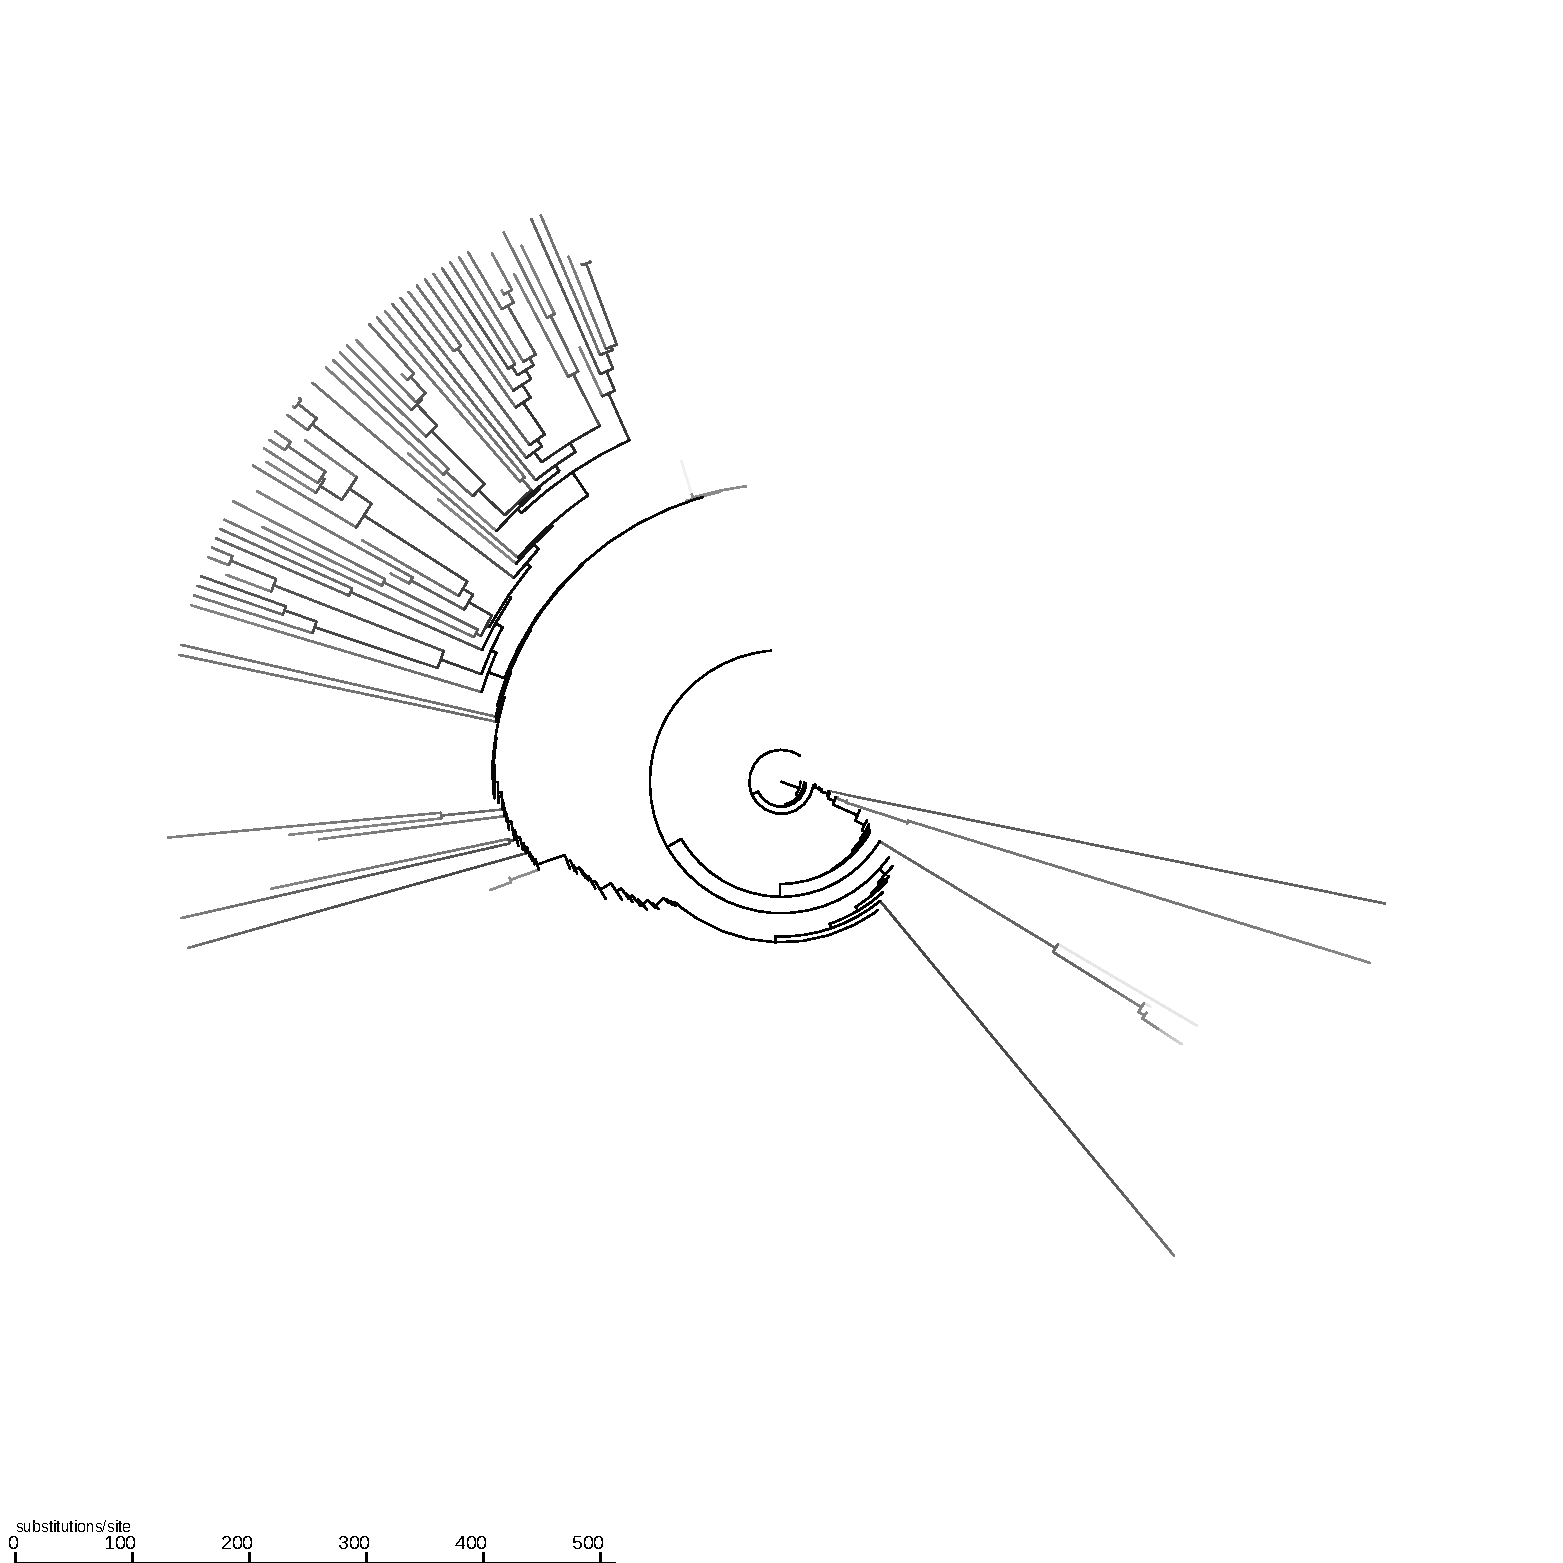
\includegraphics[scale=0.6]{tree-clust.pdf}
  \caption{An example of a tree that used the
    \emph{tree\_map\_for\_split\_set} to only highlight a certain
    family in a tree. You see the logarithmic gradient as clusters
    with few sequences are shown in light gray, while clusters
    containing the entire set of sequences, that belong to the
    outlined family are dark and black. The substitutions/site are
    again automatically generated by the Newick tools
    \cite{newick_tools} and are to be ignored.}
  \label{fig-treemapset}
\end{figure}

\subsection{Implementation}
The \emph{tree\_map\_for\_split\_set} tool is implemented in \newline
\emph{tree\_map\_for\_split\_set.c}.



        
